Kao shto se mozhe videti na slici \ref{fig:arh} postoji vishe razlichitih interfejsa u zavisnosti od uloge korisnika u sistemu. U nastavku se nalaze skice interfejsa.

\subsection{Interfejs za klijenta}
\begin{figure}[H]
    \centering
    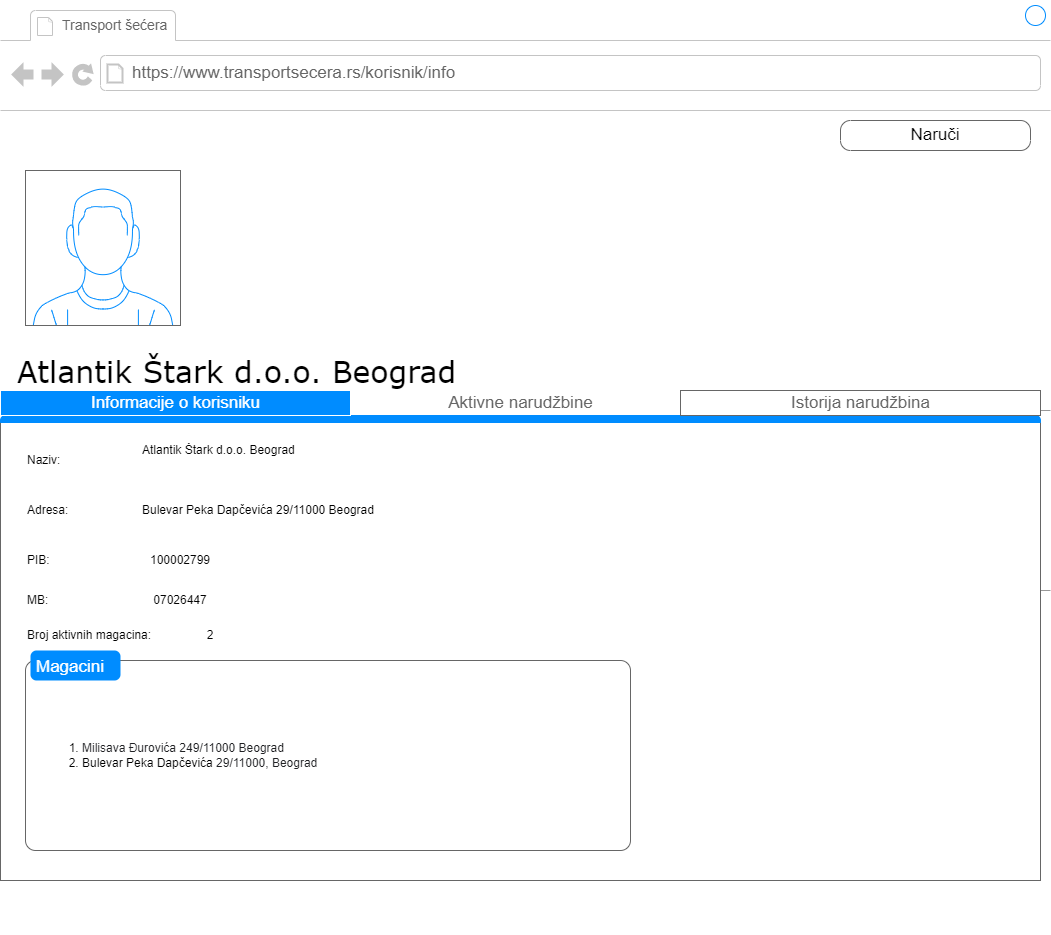
\includegraphics[scale=0.3]{Slike/KorisnickiInterfejs/Korisnik/korisnikInfo.png}
    \caption{Informacije o klijentu}
    \label{fig:klijentInfo}
\end{figure}

\begin{figure}[H]
    \centering
    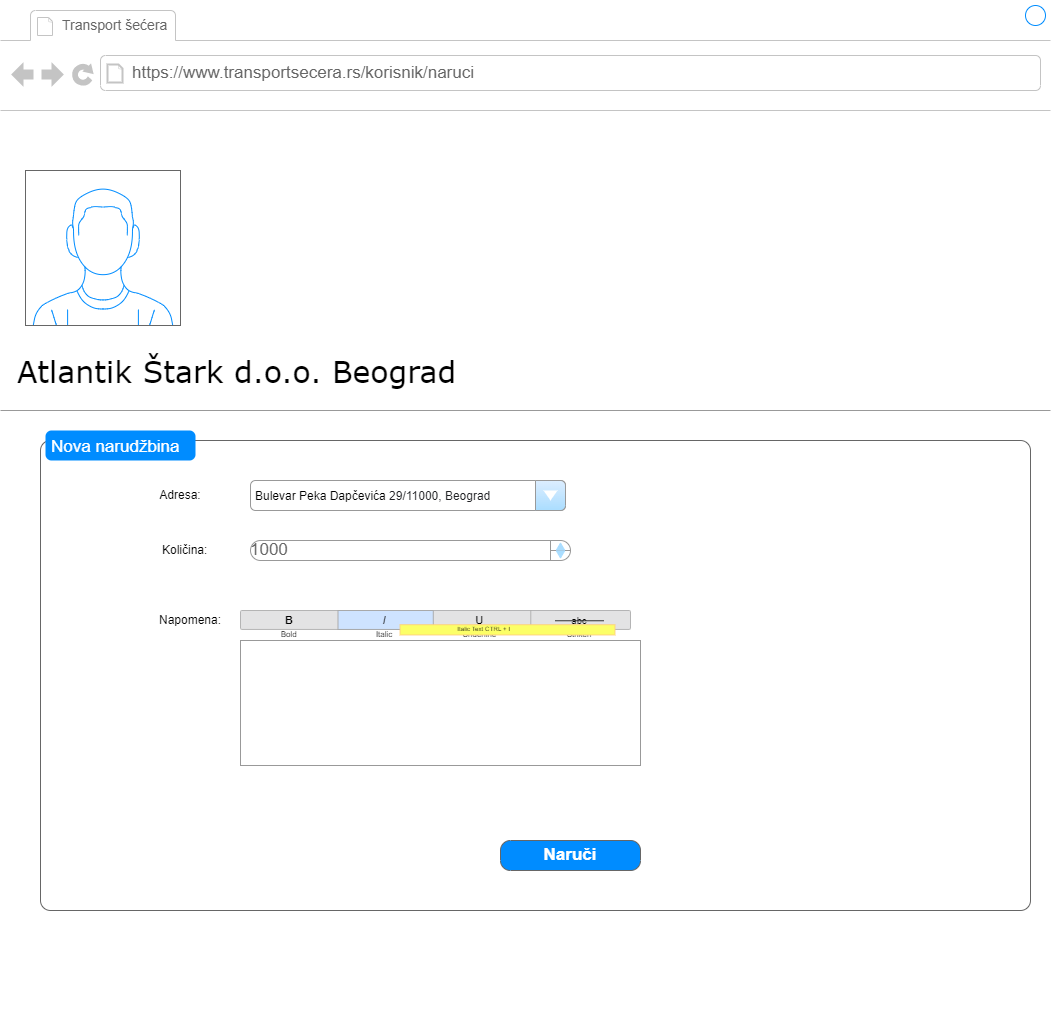
\includegraphics[scale=0.25]{Slike/KorisnickiInterfejs/Korisnik/korisnikNaruci.png}
    \caption{Slanje zahteva za transport}
    \label{fig:klijentNaruci}
\end{figure}

\begin{figure}[H]
    \centering
    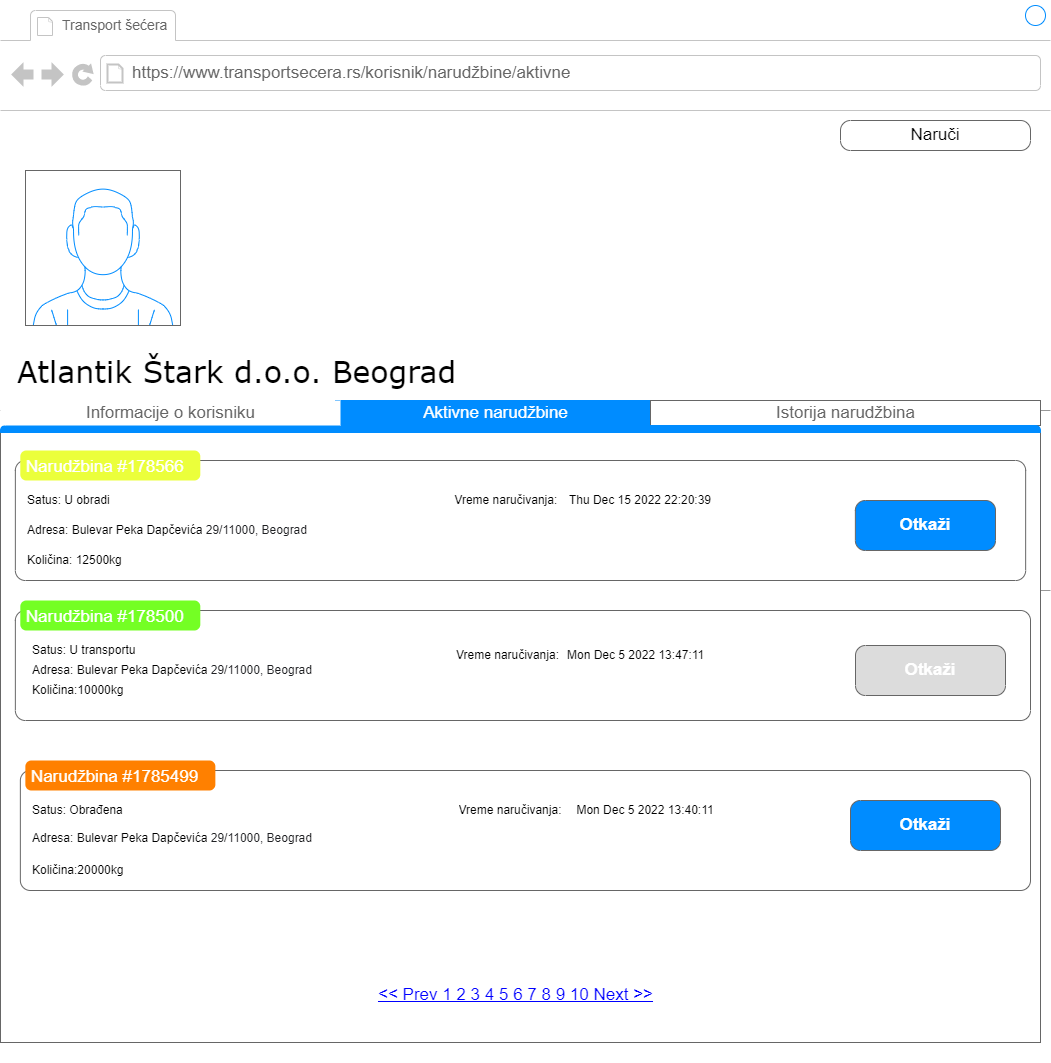
\includegraphics[scale=0.3]{Slike/KorisnickiInterfejs/Korisnik/korisnikAktivne.png}
    \caption{Pregled aktivnih zahteva}
    \label{fig:klijentAktivne}
\end{figure}
\begin{figure}[H]
    \centering
    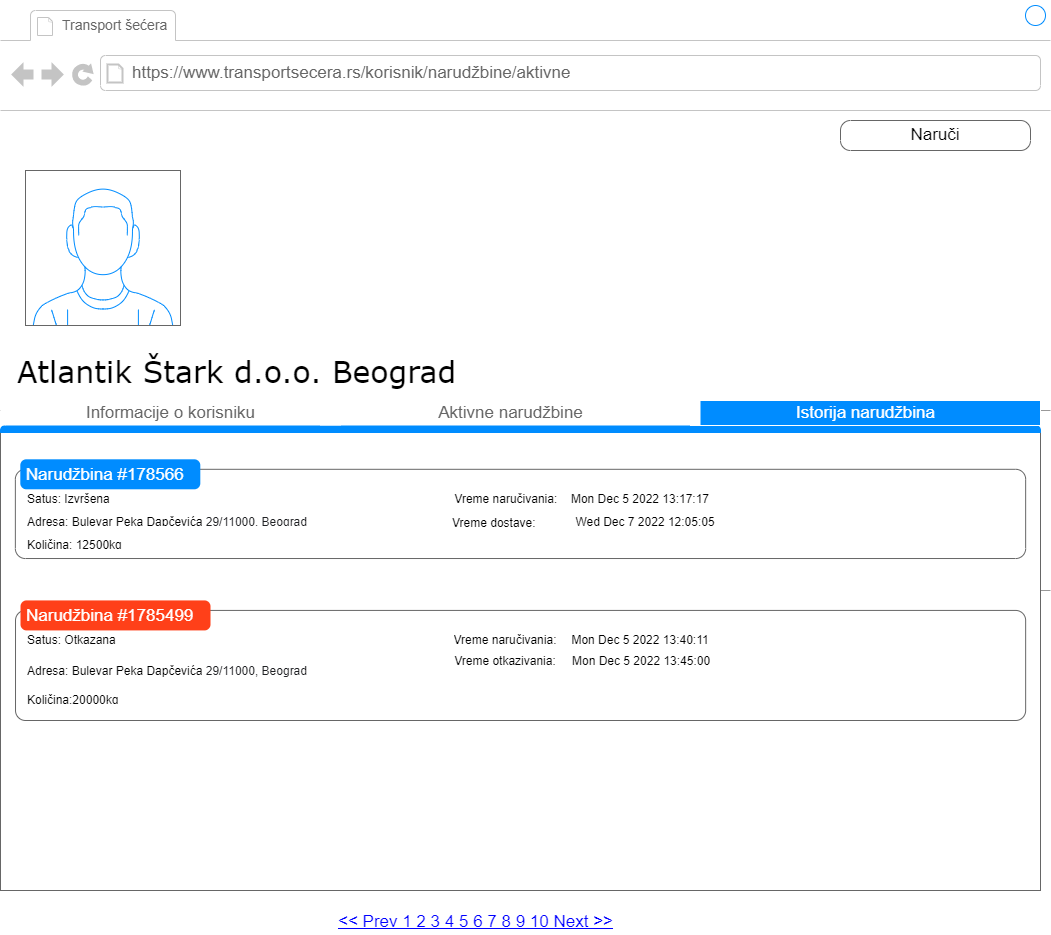
\includegraphics[scale=0.25]{Slike/KorisnickiInterfejs/Korisnik/korisnikIstorija.png}
    \caption{Pregled istorije zahteva}
    \label{fig:klijentIstorija}
\end{figure}

\subsection{Interfejs za administratora}

\subsection{Interfejs za vozache}
